%===================================== CHAP 5 =================================

\chapter{Experiments}
In order to get data to analyse and evaluate the proposed methodology, a series of experiments was performed using a small boat in the channel near Ravnkloa in Trondheim. The sensors were mounted on a rigid mount, and the boat performed a series of maneuvers in front of the sensors, in order to gather sensor data to be post-processed and analyzed. The data was saved in rosbags during the experiments, to be post-processed in ROS and MATLAB after the data gathering.

The experiments were performed at Ravnkloa in the Nidelven river in Trondheim. This location was chosen due to easy access to the waterfront via a floating dock and access to electrical power outlets for the sensors and computer, courtesy of the Trondheim harbor authorities (Trondheim Havn). Figure \ref{fig:trondheim_sentrum} shows the experimental site in a satellite photo of downtown Trondheim. The circle in figure \ref{fig:trondheim_sentrum} illustrates the area where the boat maneuvers were performed, and the arrow illustrates where the sensors were placed.
\begin{figure}[H]
	\centering
	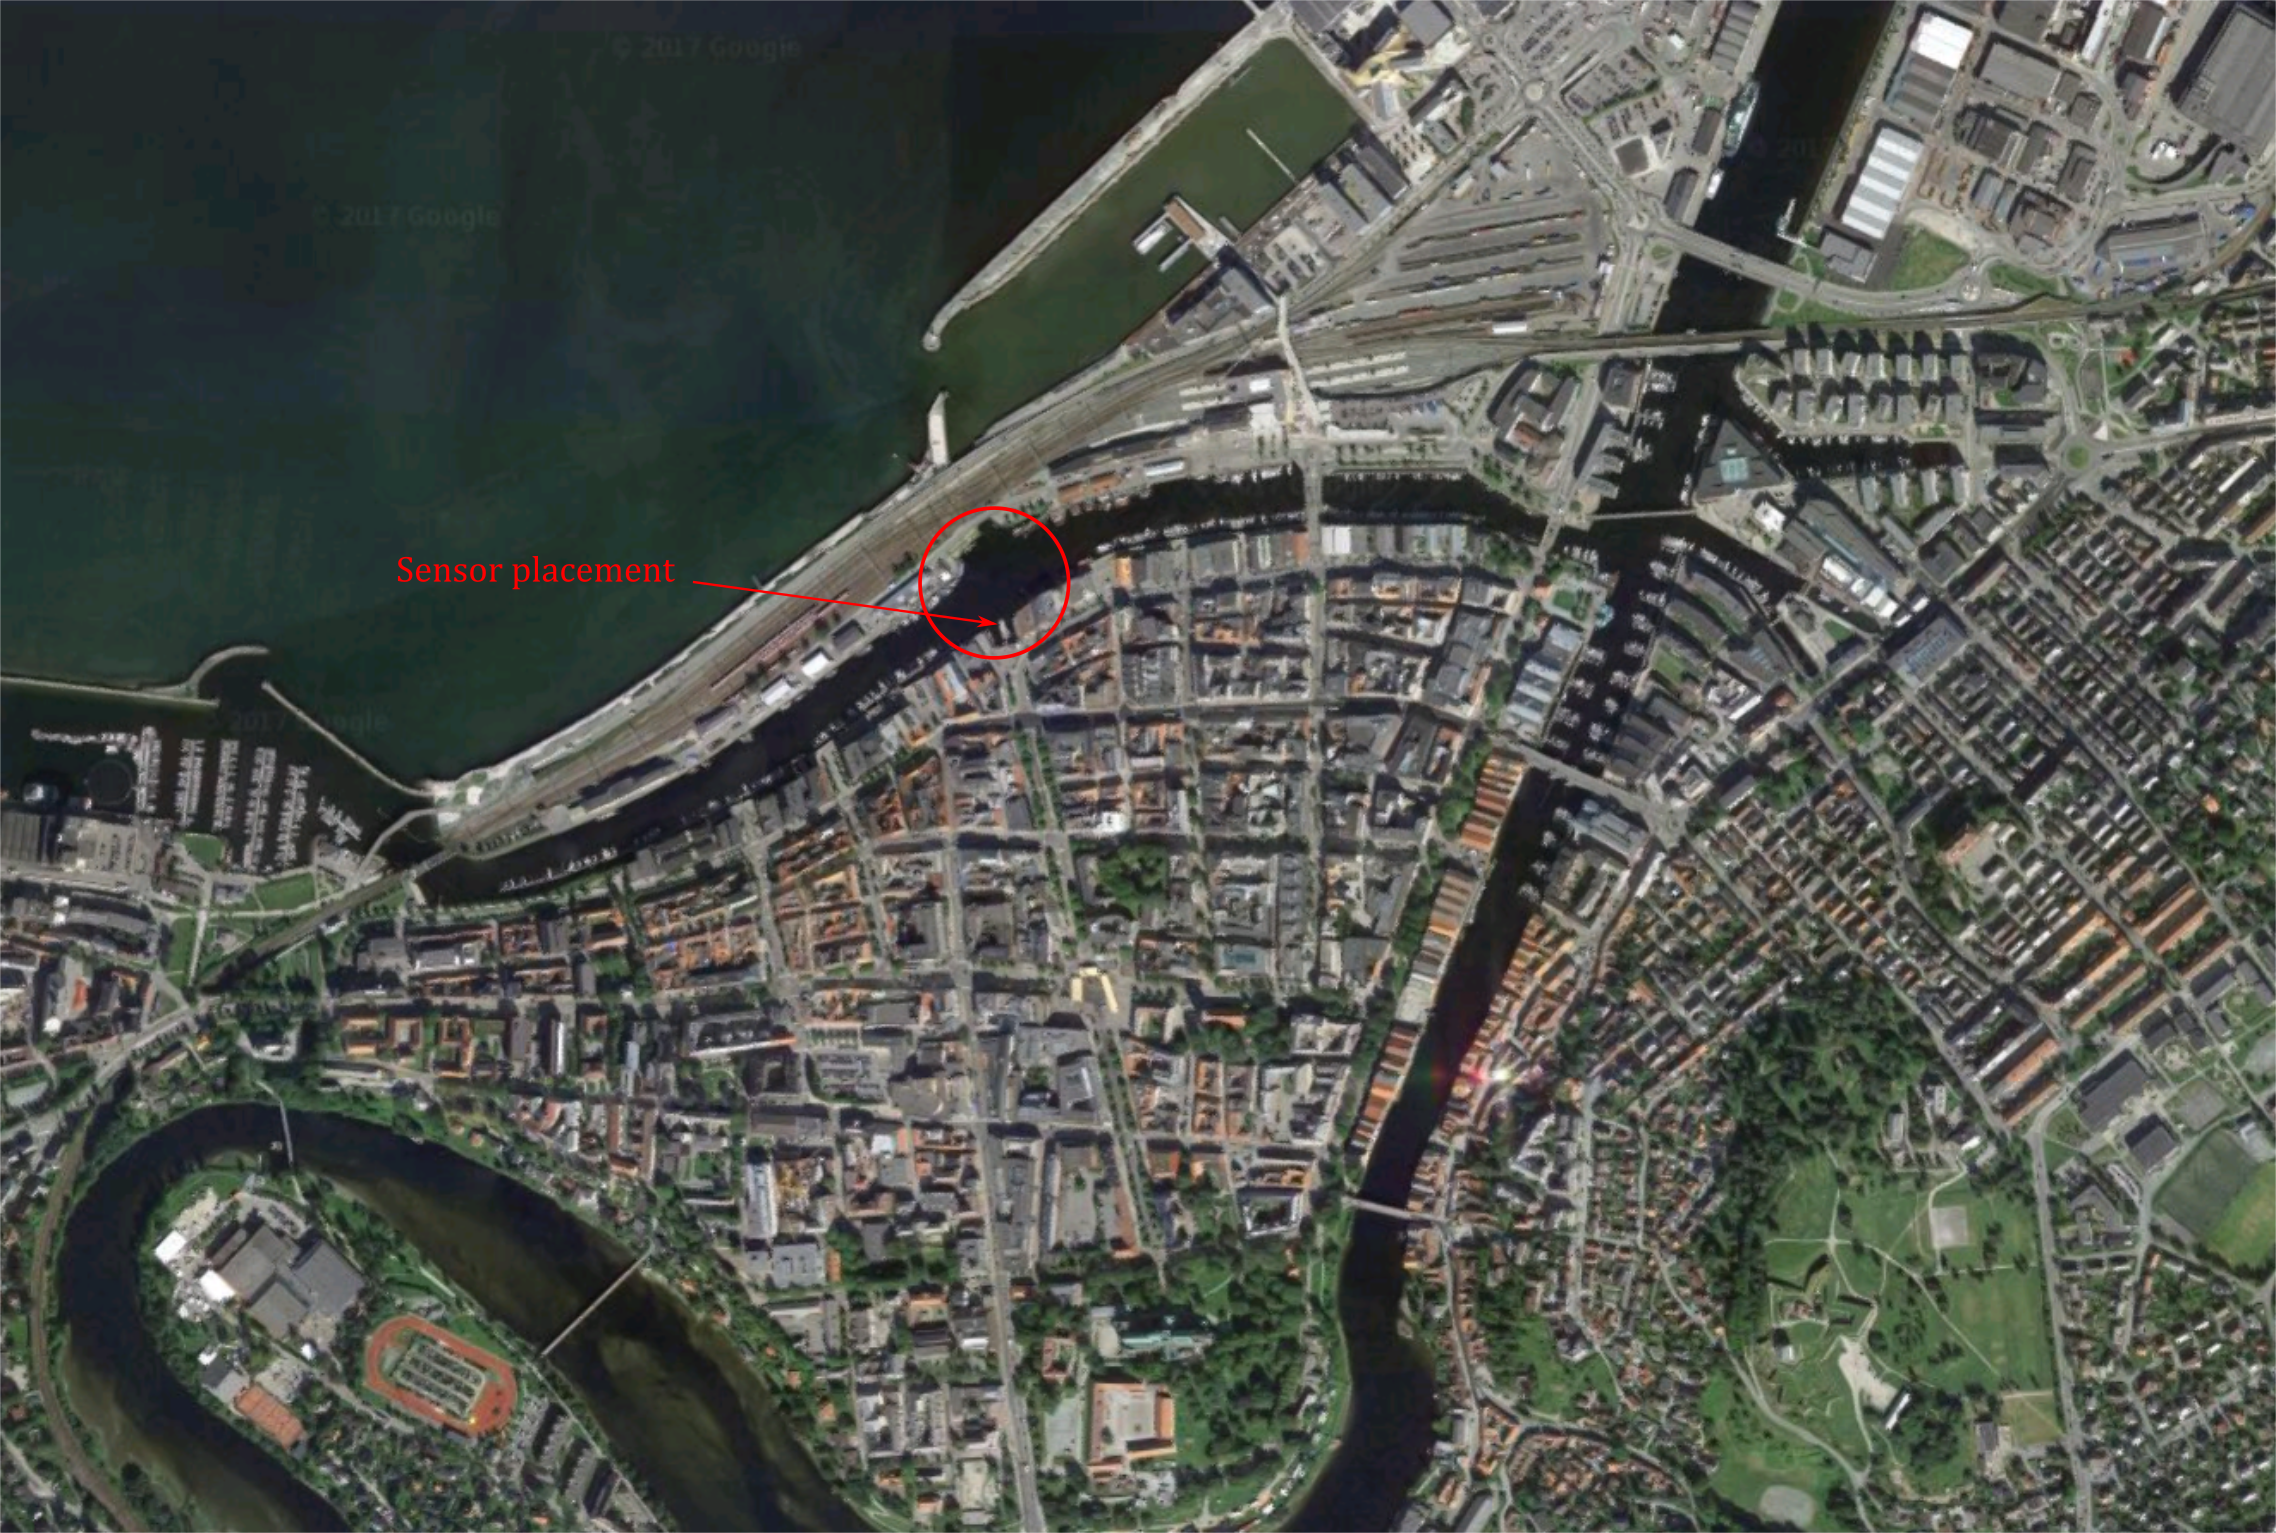
\includegraphics[width=.8\linewidth]{fig/trondheim_downtown.png}
	\caption{The experiment site in downtown Trondheim. Image taken from Google Maps.}
	\label{fig:trondheim_sentrum}
\end{figure}
The sensors were mounted on a simple rig custom made for the purpose by the workshop at NTNU ITK. Figure \ref{fig:sensors_ravnkloa} shows the sensors mounted on the rig, and the placement of the rig at the end of the floating dock at Ravnkloa.
\begin{figure}[H]
	\centering
	\begin{subfigure}{.5\textwidth}
		\centering
		\includegraphics[width=.8\linewidth]{fig/sensor_rig.jpg}
		\caption{The sensor rig, with (from the top) GNSS antenna, lidar, camera and IMU installed.}
		\label{fig:sub_sensorrig}
	\end{subfigure}%
	\begin{subfigure}{.5\textwidth}
		\centering
		\includegraphics[width=.8\linewidth]{fig/sensors_ravnkloa.jpg}
		\caption{The sensor placement at Ravnkloa.}
		\label{fig:sub_sensor_ravnkloa}
	\end{subfigure}
	\caption{The sensor rig, and its placement at the floating dock at Ravnkloa.}
	\label{fig:sensors_ravnkloa}
\end{figure}
The target boat used in the experiments is a 17 feet long leisure craft, owned by two PhD students at NTNU.
The boat is shown in figure \ref{fig:boat} (the blue boat). The relative small size of the boat makes it a good test target for the proposed system, as detection of small leisure crafts will be important from a safety standpoint when an autonomous vessel is maneuvering in confined environments and close to shore, where such crafts are typically found.
\begin{figure}
	\centering
	\includegraphics[width=.8\linewidth]{fig/experiment_boat.jpg}
	\caption{The boat used as a target in the experiments.}
	\label{fig:boat}
\end{figure}
\section{Performed Maneuvers}
In order to be able to compare detections in images with data from the lidar, and to gain insight into how well image detections of the boat corresponds to detections in the lidar point cloud, a series of maneuvers with different geometries were performed in the river around the sensor placement.
\cleardoublepage